\documentclass[11pt, aspect ratio=169]{beamer}
\usetheme{Madrid}
\usepackage[utf8]{inputenc}
\usepackage{amsmath}
\usepackage{amsfonts}
\usepackage{amssymb}
\usepackage{ragged2e}
\usepackage{array}
\usepackage{subfig}
\usepackage{animate}
\usepackage{wrapfig}
\usepackage{algorithm}
\usepackage{algorithmic}


\author[]{Shridatha Hegde (01FE18BEC171) , Akhilesh Kumbhar (01FE18BEC016),\newline  Sai Preetham (01FE18BEC146), Saiprasanna Kuragodi (01FE18BEC147),\newline Sagar Patil (01FE18BEC145) \vspace{5pt} \newline Under the guidance of \newline Dr. Sunita V.B.}

\vspace{-20pt}
\title{Non Invasive Smart Energy Monitoring System}
\setbeamercovered{transparent}

\setbeamertemplate{navigation symbols}{}
\makeatletter
\defbeamertemplate*{footline}{Dan P theme}
{
\leavevmode%
\hbox{%
\begin{beamercolorbox}[wd=.15\paperwidth,ht=2.25ex,dp=1ex,center]{author in head/foot}%
\usebeamerfont{author in head/foot}\insertshortauthor
\end{beamercolorbox}%
\begin{beamercolorbox}[wd=.55\paperwidth,ht=2.25ex,dp=1ex,center]{title in head/foot}%
\usebeamerfont{title in head/foot}\insertshorttitle
\end{beamercolorbox}%
\begin{beamercolorbox}[wd=.3\paperwidth,ht=2.25ex,dp=1ex,right]{date in head/foot}%
\usebeamerfont{date in head/foot}\insertshortdate{}\hspace*{2em}
\insertframenumber{} / \inserttotalframenumber\hspace*{2ex}
\end{beamercolorbox}}%
\vskip0pt%
}
\makeatother
%\setbeamertemplate{footline}[page number]
\logo{}
\titlegraphic{
\includegraphics[scale=0.3]{images/BVB.png}}
\institute{KLE Technological University,Vidyanagar, Hubballi-580031,Karnataka, India}
% \vspace{-15pt}
\usepackage{datetime}
\newdate{date}{17}{07}{2021}
\date{\displaydate{date}}
\subject{Project Title}
\bibliographystyle{plain}
\begin{document}

\begin{frame}
\titlepage
\end{frame}

\begin{frame}{Contents}
\begin{itemize}
\item Introduction
\item System Design 
\item Implementation details
\item Results
\item Conclusion
\end{itemize}
\end{frame}

\begin{frame}{Introduction}
\begin{center}
\begin{large}
% \textbf{Introduction}
\begin{itemize}

\item Using energy efficiently in smart homes saves money,enhances sustainability and reduces carbon footprint.
\item Consumer electronics, office equipment and other plug loads consume 15 to 20 percent of total residential and commercial electricity while not in primary mode. Much of this energy is consumed when these devices operate in low-power modes but are not actually in use.
\item One way to reduce this unnecessary electricity consumption is to use a smart energy monitoring system.

\end{itemize}
\end{large}
\end{center}
\end{frame}


\begin{frame}{Motivation}
\begin{itemize}
	\item The electricity bill generated by the electricity supply company can be often confusing as it does
not explain the consumption of individual rooms or labs or cabins but instead, the bill provides a sum of all these as a whole. So this project as a whole tries to explain the power consumed individually by these sections. 
	\item Predicting the possible power consumption is a very important job at hand as this helps to plan the consumption accordingly. Using different machine learning algorithms, these possible future values would be sought.
\end{itemize}
\end{frame}


\begin{frame}{Objectives}
\begin{itemize}
	\item To design and develop a data acquisition system for measuring energy consumption
	\item To Visualize and forecast consumption usage with cloud computing
	\item To make energy monitoring smarter
\end{itemize}
\end{frame}


\begin{frame}{Literature Survey}
\textbf{Literature survey related to the project}
\begin{itemize}
	\item \underline{Paper 1} An Internet of Things Framework for Smart Energy in Buildings: Designs, Prototype, and Experiments
	\begin{itemize}
		\item A novel experimental prototype IoT system which demonstrates the real time location-based automated energy policy control across multiple buildings.
        \item Transforming from the centralized control and static energy consumption modes to distributed and dynamic energy control in the consumer-side smart grids containing various common buildings.
	\end{itemize}
	\item \underline{Paper 2}- Machine learning based system for managing energy efficiency of public sector as an approach towards smart cities
	\begin{itemize}
		\item Incorporating Big Data platform and machine learning into an intelligent system for managing energy efficiency of public sector as a substantial part of the smart city concept.
		\item Deep neural networks, Rpart regression tree and Random forest with variable reduction procedures were used to create prediction models.
	\end{itemize}
\end{itemize}
\end{frame}



\begin{frame}{Problem Statement}
\centering
\textbf{To design and develop a non-invasive smart energy monitoring system.}
\end{frame}


\begin{frame}{System Design}
 \begin{figure}[H]%[!ht]
\begin {center}
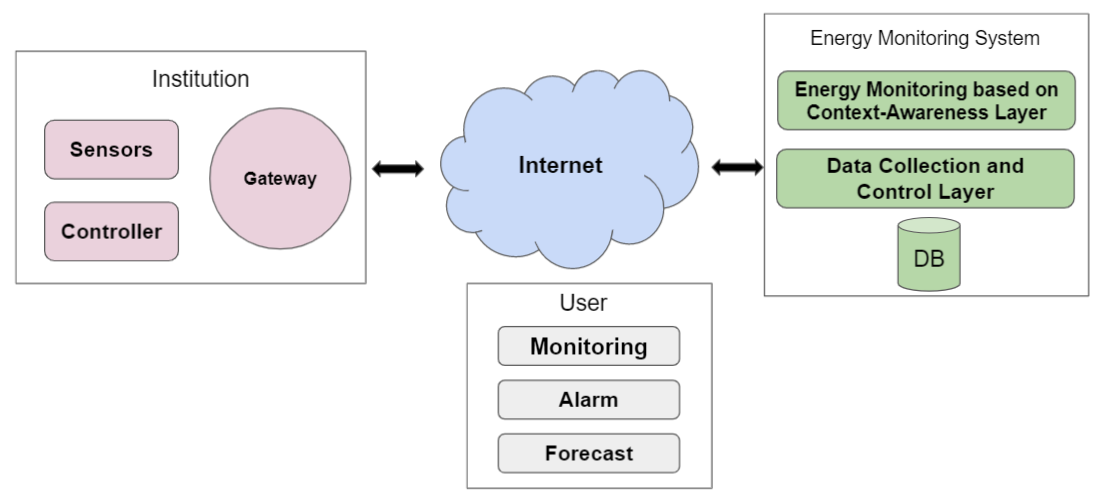
\includegraphics[width=8.5cm=\textwidth]{images/flow1.png}
\caption{Proposed system design for the institution}
\end {center}
\end{figure}
% \textbf{Discuss the overview of the block used in the project.}

\end{frame}




% \begin{frame}{Proposed  Design}
% \begin{figure}[h!]
% \centering
% 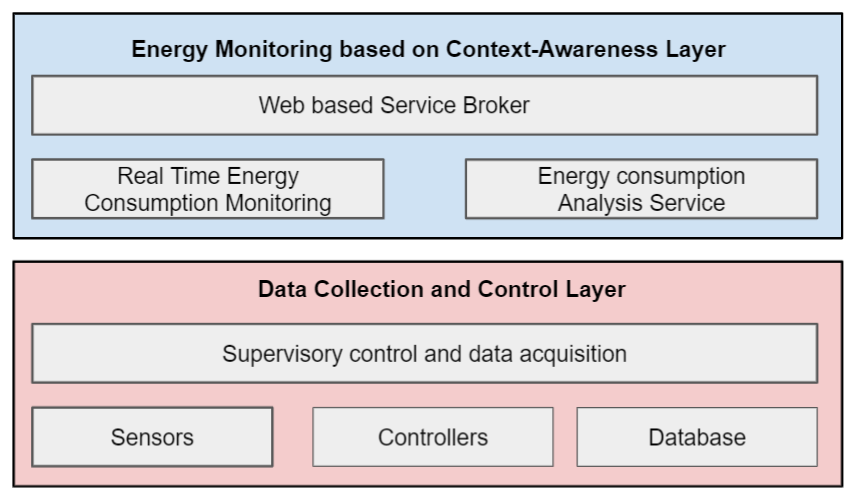
\includegraphics[width=8cm,height = 5cm,frame]{problock.png}
% % \caption{The proposed energy monitoring block diagram with first layer based on context awareness and second layer as data collection control.}
% % \label{fig:Proposed Block Diagram of system}
% \end{figure}
% \end{frame}

\begin{frame}{Algorithm}
 \begin{figure}[H]%[!ht]
\begin {center}
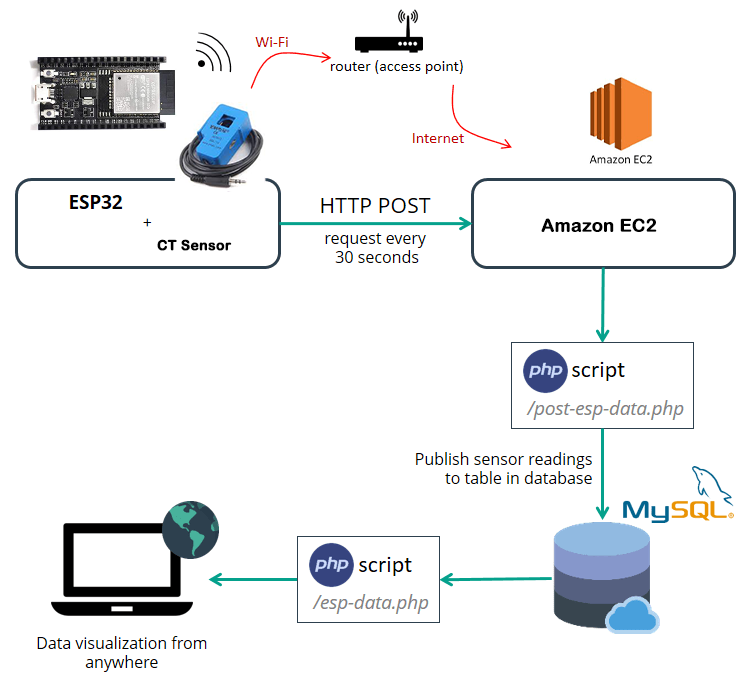
\includegraphics[width=7cm=\textwidth]{images/framework.png}
\caption{Configuration flow for the energy monitoring}
\end {center}
\end{figure}
\end{frame}

\begin{frame}{Hardware Implementation }
\begin{center}
\begin{large}
% \textbf{Implementation Details}
\end{large}
\end{center}
% \textbf{Circuit diagram}
\begin{figure}[h!]
\centering
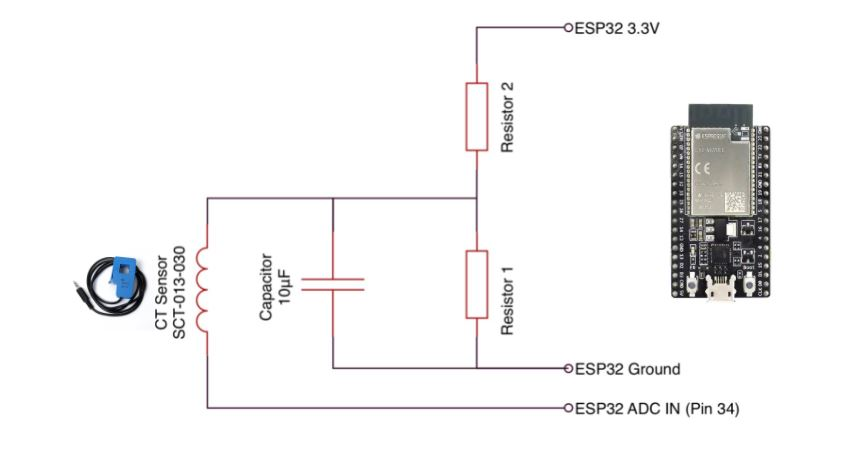
\includegraphics[width=10cm=\textwidth]{images/circuitf.JPG}
\caption{Circuit diagram}
\end{figure}
\end{frame}

\begin{frame}{Forecast Model Implementation}
\begin{itemize}
    \item 3D tensor input shape
    \item Intermediate stacked LSTM layers 
    \item Dropout layer
    \item Dense layer
\end{itemize}
% \begin{figure}[h!]
% \centering
% \includegraphics[width=8cm=\textwidth,frame]{model2.png}
% \caption{Stacked Lstm Architecture}
% \end{figure}

 \begin{table}[]
\centering
  \begin{tabular}{||c|c|c||}
  \hline
     \textbf{Layer (type)}  &  \textbf{Output Shape} & \textbf{Parameters}\\ [0.5ex]
  \hline\hline   
     lstm\_20 (LSTM)  &  (None,90,60) & 14880\\
  \hline   
     lstm\_21 (LSTM)  &  (None,60) & 29040\\
  \hline 
     dropout\_10 (Dropout) & (None,60) & 0\\
  \hline
     dense\_19 (Dense) & (None,1) & 61\\ [1ex]
\hline
  \end{tabular}
  \end{table}

\end{frame}

\begin{frame}{Optimization}
\begin{itemize}
    \item \textbf{{Power Saving}}-
    In \textit{Light sleep mode} the CPU is halted by turning off its clock pulses, while the RTC and ULP-coprocessor remain functioning.
    \item \textbf{{Deep learning Hyper-parameter Tuning}}-
    \begin{figure}[h!]
    \centering
    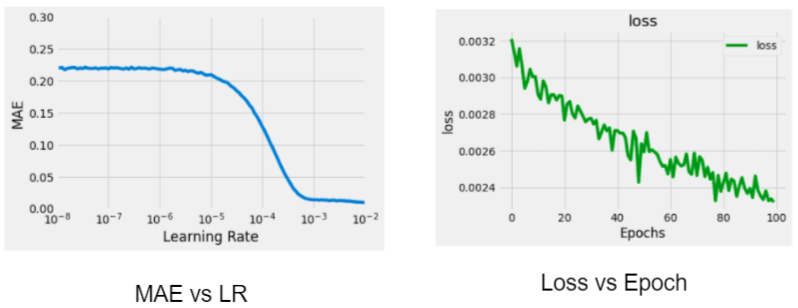
\includegraphics[width=10cm=\textwidth]{images/hyper.png}
    %\caption{Learning rate and Epochs Trade-off}
    \end{figure}
    
\end{itemize}
\end{frame}

\begin{frame}{Results}
     \begin{figure}[H]%[!ht]
\begin {center}
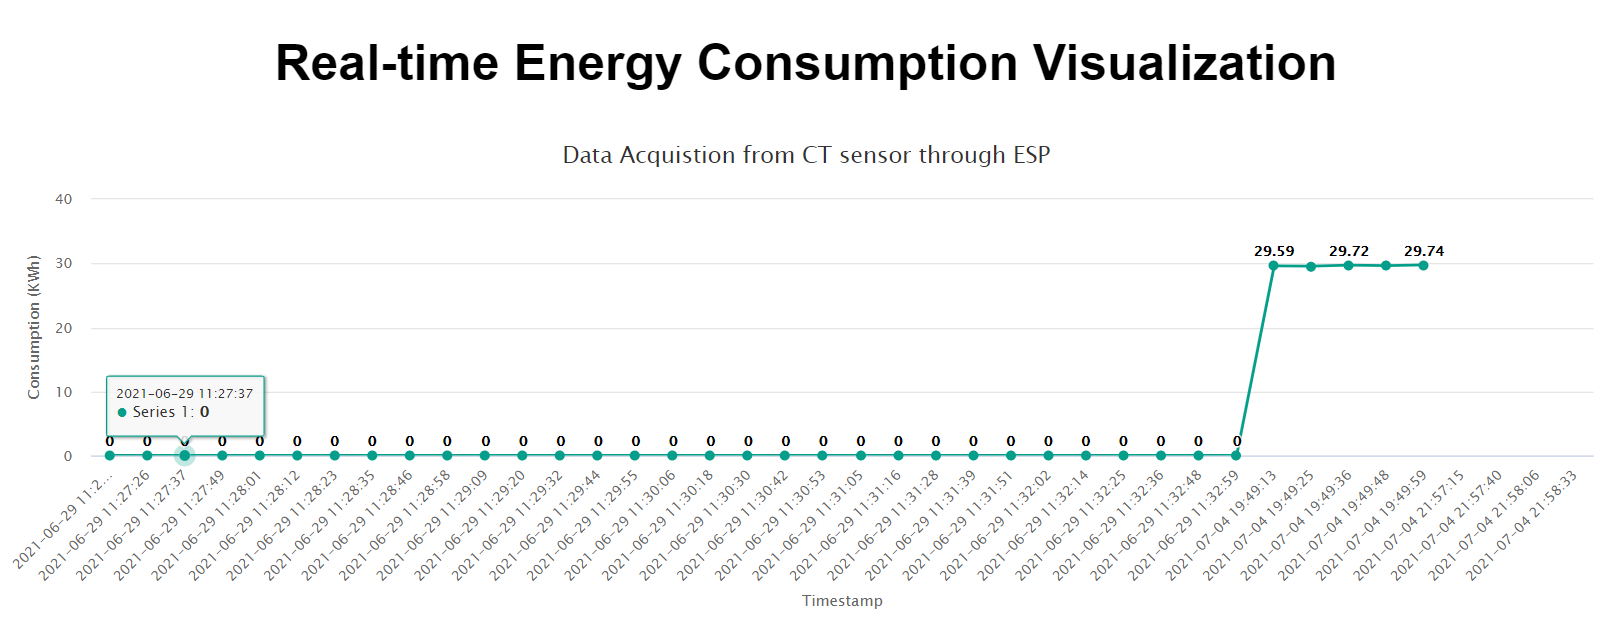
\includegraphics[width=12cm,height=6cm]{images/dashboard.png}
\caption{Real-time visualization of Energy Consumption}
\end {center}
\end{figure}
\end{frame}


\begin{frame}{Results}
         \begin{figure}[H]%[!ht]
            \begin {center}
            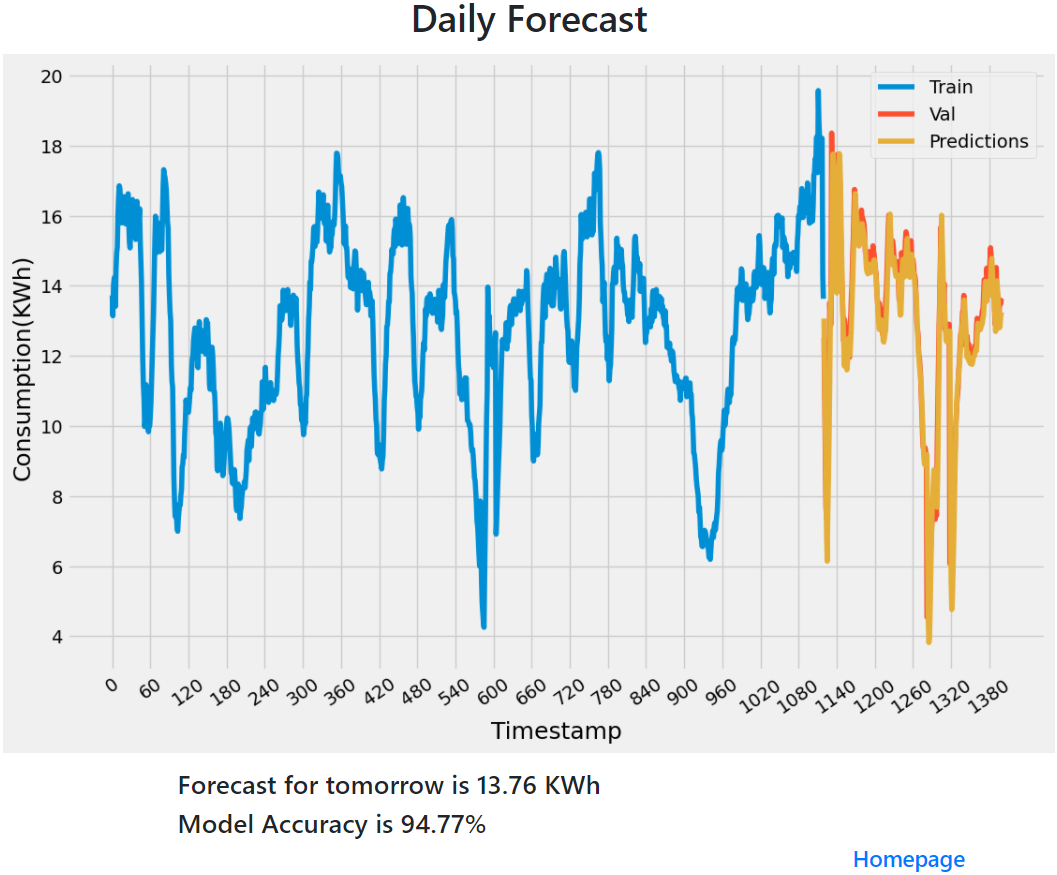
\includegraphics[width=10cm,height=6cm]{images/results.png}
            \caption{Web-app for Forecast model based on LSTM}
            \end {center}
            \end{figure}
\end{frame}


\begin{frame}{Discussion on Results}
\begin{itemize}
    \item The hardware implementation requires a current sensor to measure the current consumption and a Node MCU to accept the values from the sensor and send the generated data to the database.
    \item The data acquired from the node sensor is of Time Series nature.
    \item The product conceptualized by the team has tremendous potential of visualizing the power consumption  of a particular place with an accuracy of about 95\%.
\end{itemize}
 
\end{frame}


\begin{frame}{Future Scope}
% Following features can be conceptualized as scope for the extension of the project- 
 \begin{itemize}

  \item Automatically recognize anomalies in the appliances based on their consumption pattern. 
  \item Tweak the GraphQL API 
%\item[$\cdot$ ]Investigate if we could put the ESP32 inside the electrical box on a DIN rail
 \item Integrate with Google Home 
 \item Multiple model deployments providing versatile predictions.
 \end{itemize}
 \end{frame}

\begin{frame}{Thank-You}
\begin{center}
\begin{large}
\textbf{Thank-You}
\end{large}
\end{center}
\end{frame}

\end{document}